\documentclass{report}
\usepackage{geometry} % Page layout
\usepackage{multicol,caption} % Multiple columns
\usepackage{fancyhdr}
\usepackage{titlesec} % Section formatting
\usepackage{setspace} % Setting line spacing
\usepackage[backend=biber,style=apa,citestyle=authoryear]{biblatex}

\usepackage{lipsum} % dummy text

\renewcommand*{\nameyeardelim}{\addcomma\space}
\DeclareDelimFormat[parencite]{finalnamedelim}{\addspace\&\space}
\addbibresource{references.bib}

\newenvironment{Figure}
  {\par\medskip\noindent\minipage{\linewidth}}
  {\endminipage\par\medskip}

\geometry{landscape, margin=0.5in}
\setlength{\columnsep}{1cm}
\setlength{\columnseprule}{0.5pt}
\pagenumbering{gobble}

\pagestyle{fancy}
\lhead{Jayden Lefebvre}
\rhead{SAFS3530 Trent University}
\setlength{\headheight}{36pt}

\titleformat{\section}{\normalfont\fontsize{12}{15}\bfseries}{\thesection}{1em}{}

\begin{document}

\begin{center}
  \Large
  Ethylene Exposure and Growth Rate in Early Vegetation of \textit{Narcissus sp.}
\end{center}

\vspace{0.5cm}

\begin{multicols}{3}

  \section*{Abstract}
  The effect of different concentrations of ethylene on plant bulb phenology is investigated.
  Apples are used as a source of ethylene gas in a closed greenhouse system.
  Bulb leaf height is measured over a period of one month.
  Leaf growth and growth rate are compared between control and ethylene-treated groups, and final leaf height is correlated with ethylene concentration.
  Results were largely inconclusive, indicating poor experimental design or the influence of outside factors.
  \section*{Introduction}
  Ethylene is a plant growth regulator responsible for fruit ripening and cell senescence.
  It has been reported in literature that exposure to ethylene can negatively impact plant shoot elongation in bulbous plants \parencite{bulbous}, and even induces leaf abscission (i.e. death) after long periods of exposure \parencite{abscission}.
  Literature findings indicate that the mechanism underlying these phenomena relate to the inhibition of auxin synthesis or enhancing auxin destruction \parencite{senescence}.
  It is hypothesized that ethylene will negatively influence leaf height in plant bulb vegetation.
  \vfill\null
  \columnbreak
  \section*{Methods}
  % Each apparatus will have 1: pot (with soil and bulb), apple (excluding the control), skewer, cover and 2-4 elastic bands. The set-up apparatus will be a closed system that will contain the ethylene given off by the apple. Each plant pot and bulb is under one cover acting as a mini-greenhouse.
  Bulbs of \textit{Narcissus sp.} are planted in pots with soil.
  Each pot is covered with a plastic cover, and an apple is placed inside the cover.
  The covered pot acts as a closed system to contain the ethylene given off by the apple.
  Ethylene concentration is measured at day 7.
  Leaf height is measured using calipers on a weekly basis for one month.
  \section*{Results}
  Below are two graphs: Figure 1 shows the average leaf height over time per ethylene treatment group (Control, Low ethylene, and High ethylene), each with linear regression; Figure 2 shows the final (day 35) leaf height vs ethylene concentration at day 7, with linear regression and coefficient of determination.
  \begin{Figure}
    \centering
    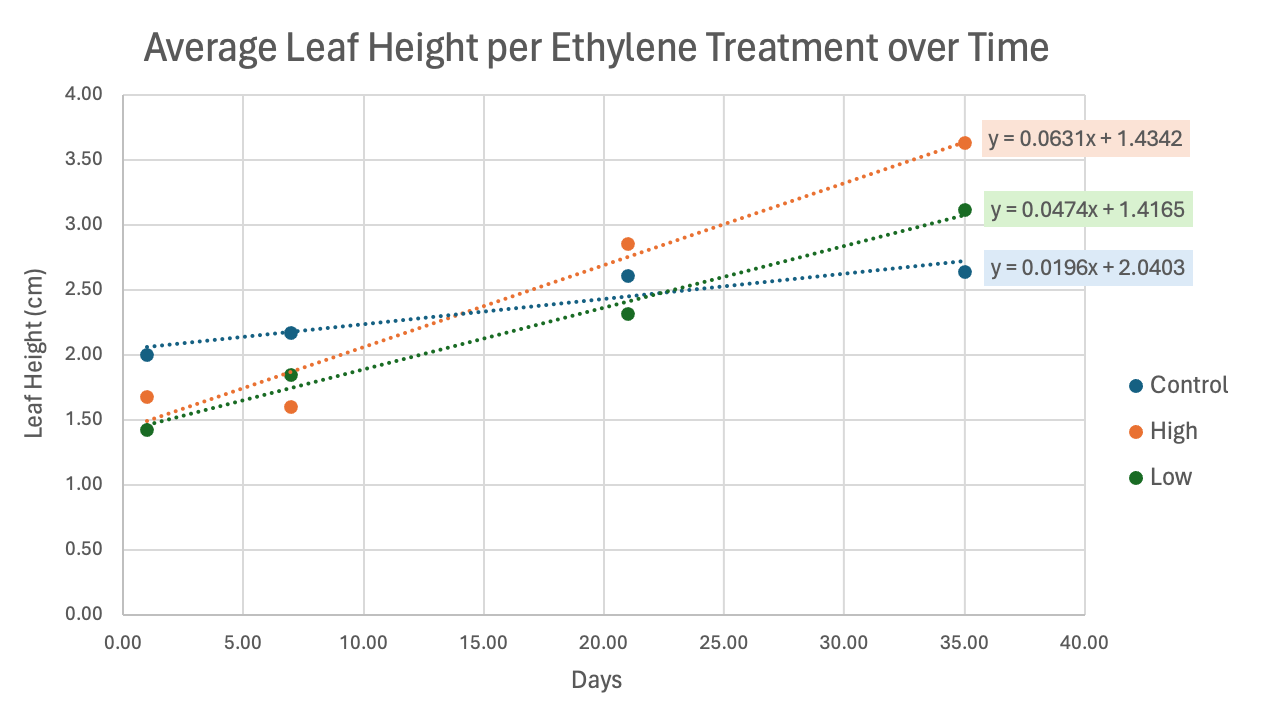
\includegraphics[width=\linewidth]{graph1.png}
    \captionof{figure}{Average leaf height per ethylene treatment in \textit{Narcissus spp.} vegetation over time.}
  \end{Figure}
  \vfill\null
  \columnbreak
  \begin{Figure}
    \centering
    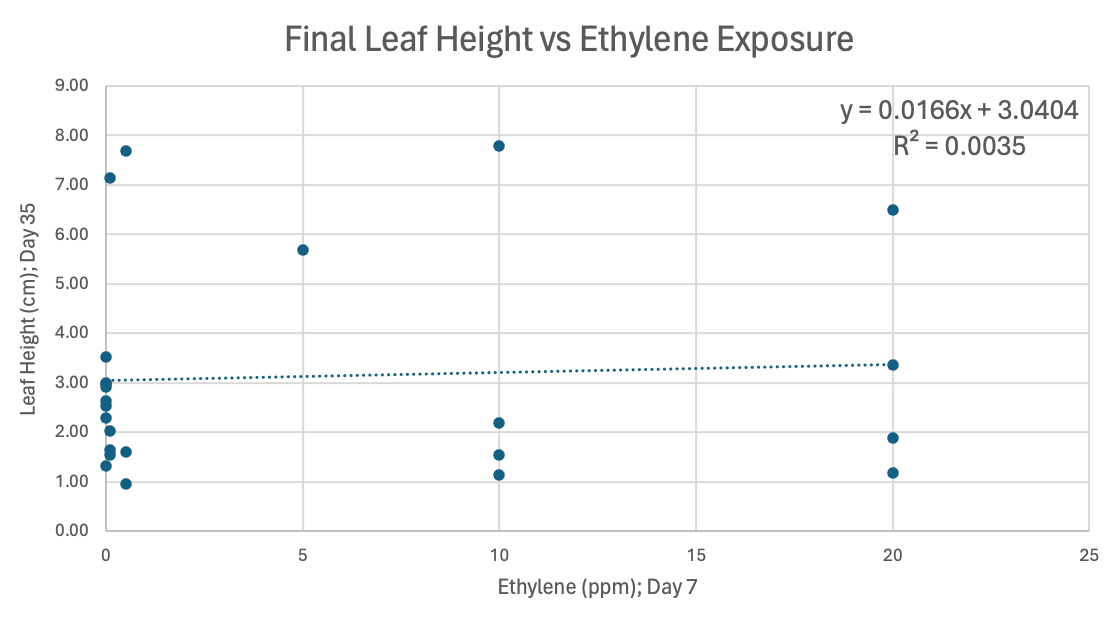
\includegraphics[width=\linewidth]{graph2.png}
    \captionof{figure}{Final (Day 35) leaf height vs ethylene concentration (Day 7) in \textit{Narcissus spp.} vegetation.}
  \end{Figure}
  \section*{Discussion}
  Increasing ethylene exposure did not exhibit significant negative impact on final leaf height; no clear trend was observed (R\textsuperscript{2} = 0.0035; Figure 2). In fact, the regression slope was slightly positive, indicating a slight increase in leaf height with increasing ethylene concentration. This is corroborated by data from Figure 1, which showed that ethylene-treated plants grew faster and had a higher final leaf height on average than control. While these findings initially suggest that ethylene may have a positive effect on plant growth, it is more likely that the results are due to poor experimental design or the influence of outside factors. Future research should focus on increasing the amount of data collected on ethylene concentrations, and running the experiment for a longer period of time.
  
\end{multicols}

\clearpage

\setstretch{1.5}

\printbibliography

\end{document}